\startfirstchapter{Introduction}
\label{chapter:introduction}

The Standard Model (SM) of particle physics is the most complete theory that exists to describe elementary particles and their interactions. However there are known weaknesses in the SM, one of which is the failure to include a description of dark matter (DM). There is strong evidence from astronomical observations that there is a large excess of matter in the universe that appears to have only gravitational interactions with SM particles. Some examples for the evidence of dark matter include measurements of rotation velocities of spiral galaxies, gravitational lensing effects, and anisotropies in the cosmic microwave background. The standard model of cosmology predicts that dark matter accounts for more than 80\% of the total matter in the universe. Although there are many theories to describe possible dark matter candidates, the one of interest here is the WIMP (weakly interacting massive particle). The WIMP is a Dirac fermion, often denoted $\chi$, and is predicted to interact gravitationally and through other force(s), potentially beyond the SM. It is believed to have a mass between $\mathcal{O}(1)$ GeV and $\mathcal{O}(100)$ TeV and have a self-annihilation cross section similar to that of SM weak interactions \cite{Bertone:2017adx}.

There are three categories of experiments that have potential to observe dark matter: direct detection, indirect detection, and collider production. Figure \ref{fig:detection} shows a schematic that illustrates their complementarity to one another. Direct detection experiments attempt to observe recoils in SM particles from scattering with dark matter. Indirect detection experiments measure decay products from DM annihilation. Collider experiments look for dark matter that is produced from the interaction of SM particles. This work focuses on the production of dark matter at the Large Hadron Collider (LHC) using data collected from proton-proton (\pp) collisions inside the ATLAS detector.

\begin{figure}[htb]
\centering
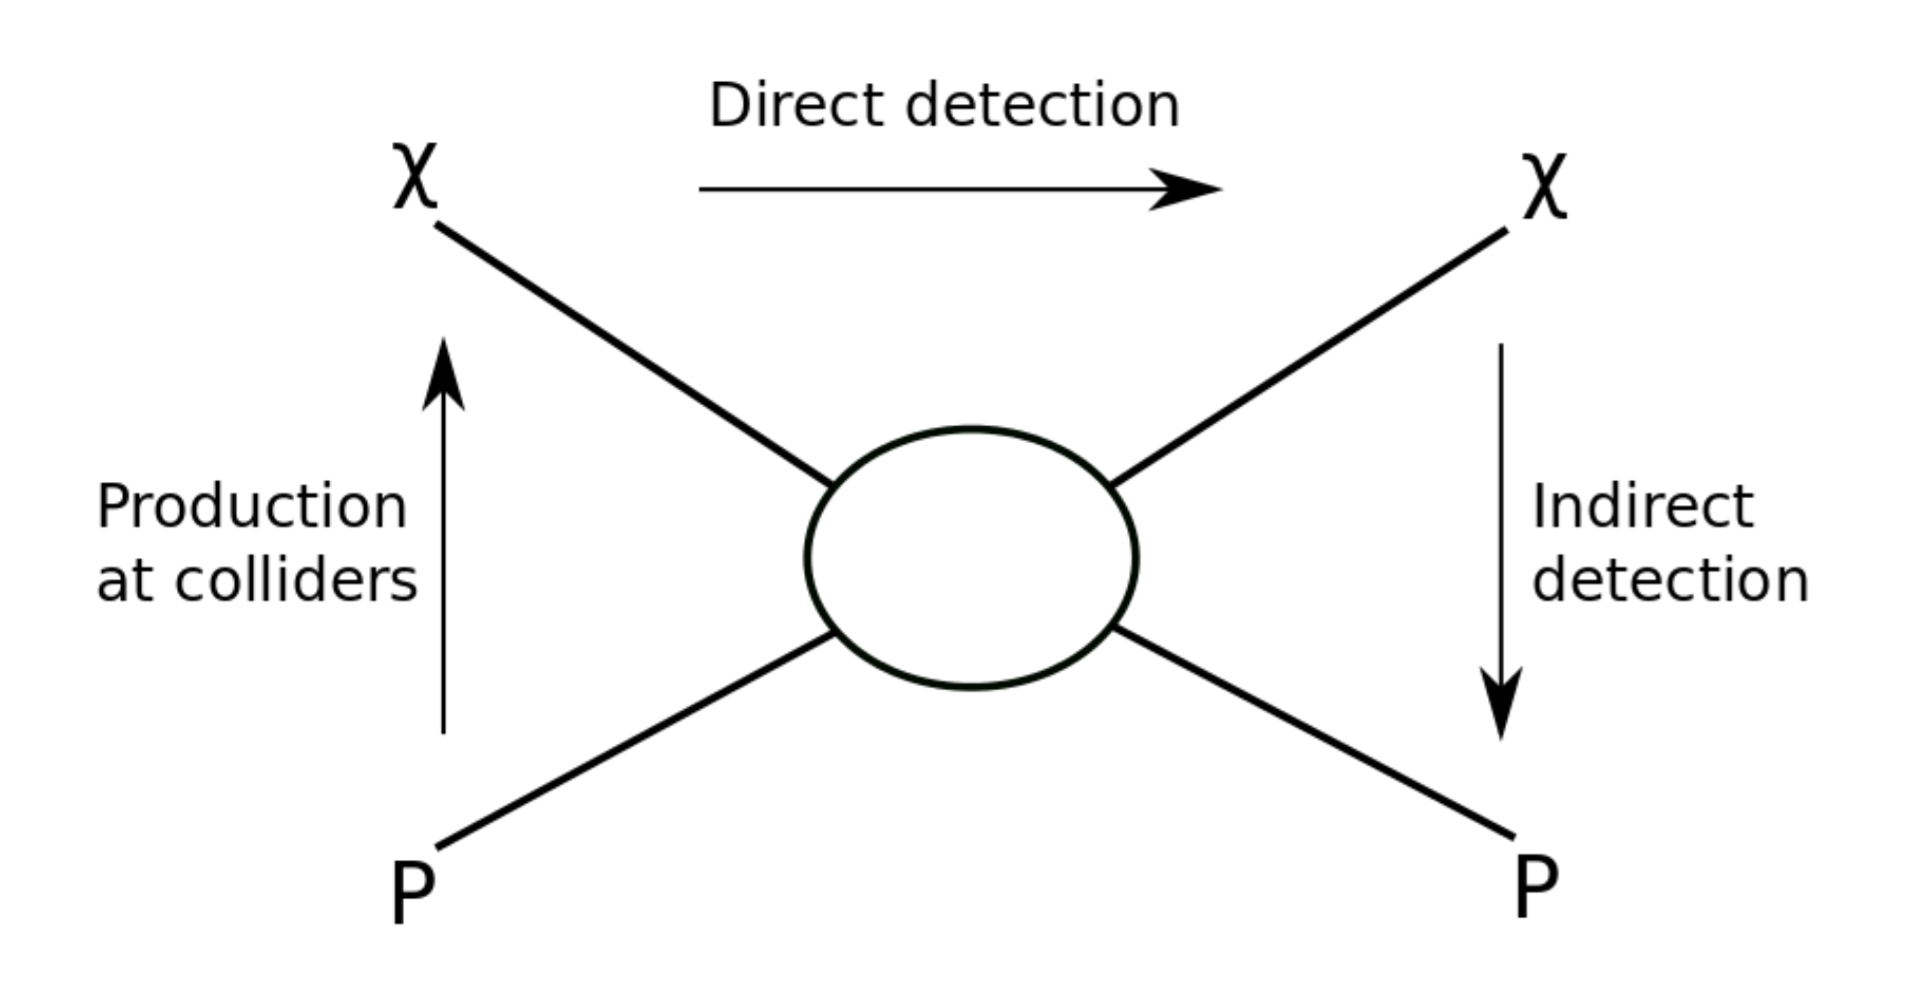
\includegraphics[width=0.6\textwidth]{Figures/detection.png}
\caption{Schematic of dark matter searches \cite{Undagoitia:2015gya}.}
\label{fig:detection}
\end{figure}

If it is possible to produce dark matter in collisions of SM particles, then an additional complication is how the presence of dark matter can be determined in the complex events of high energy particles. Collider experiments use a quantity known as missing transverse momentum, commonly denoted \etmissvec, to quantify the amount of invisible decay products in collisions. Its magnitude, \etmiss, is known as missing transverse energy. The plane perpendicular to the beam axis, also known as the transverse plane, is of particular importance in collider experiments. Before colliding, the protons in the beam only move along the beam axis, so the net momentum in the transverse plane is zero. From conservation of momentum, the net transverse momentum after the collision therefore must also be zero. If the transverse momenta of all visible particles produced in the collision are added together vectorially, they should add to zero. But, if invisible particles are present, such as neutrinos or dark matter, then the sum will instead add to a non-zero transverse momentum vector. We therefore infer that there are non-interacting particles produced, and they have a net \etmissvec that is the negative of the vectorial sum of the transverse momenta of the visible particles. Hence a dark matter signal would manifest as an excess of collision events with a significant amount of \etmiss compared to the SM prediction.

Mono-$X$ searches study a certain phenomenology of dark matter where a visible particle, $X$, is used as a `tag.' If the amount of missing energy in an event is large, the tag particle will experience a significant amount of recoil against the \etmissvec. This gives a mean of identifying potentially interesting events. In this work the \Z boson is used as a tag, which is identified in events from a pair of same sign, opposite charge leptons (\epem or \mpmm). Hence this analysis attempts to find dark matter with \Zlletmiss events, and is therefore commonly referred to as the \monoZll search. Other mono-$X$ searches use different SM particles as tags, such as a jet, photon, $W$, or the Higgs.

The ATLAS experiment has been in a period of intense data-taking since the start of Run 2 in 2015, with \pp collisions at a centre-of-mass energy of 13 TeV. As data continues to be collected until the end of 2018, the discovery potential for dark matter at the LHC has never been higher. This document summarizes the work done on the \monoZll analysis so far as well as the prospects using the full Run 2 dataset. Chapter \ref{chapter:theory} includes a summary of the dark matter models considered in the analysis, as well as a brief description of the LHC and the ATLAS detector. Chapter \ref{chapter:prevWork} covers the details of the search with a focus on the work done for the results obtained using the 2015 and 2015+2016 datasets. Chapter \ref{chapter:fullRun2} describes the plan to analyze the complete Run 2 dataset corresponding to the full 2015-2018 period.


